\section{Ergebnisse}

Nachfolgend werden für beide Spiele jeweils die Ergebnisse der Spielstanderkennungsalgorithmen an einem Beispiel präsentiert. Solange der Roboter in seiner kalibrierten Position vor dem Tablet steht und dieses nicht durch direktes Licht zu viel Spiegelung auf dem Bildschirm erzeugt, sind diese Ergebnisse repräsentativ und reproduzierbar. Sollten Spiegelungen oder anderes Rauschen zu Problemen bei der Erkennung führen, so können die nachfolgend gezeigten Bilder innerhalb der Ausführung durch Angabe der entsprechenden \textit{Debug}-Parameter angezeigt werden, um Rückschlüsse auf das Verhalten zu gewinnen. Meist genügt bei Artefakten im Bild ein Anpassen der Bilderarbeitungsroutine \vref{image_processing_routine} und hier speziell die Größe des Gaussfilters und der obere Schwellenwert des \textit{Canny}-Operators.

\subsection{TicTacToe}

\begin{figure}[!htbp]
    \centering
    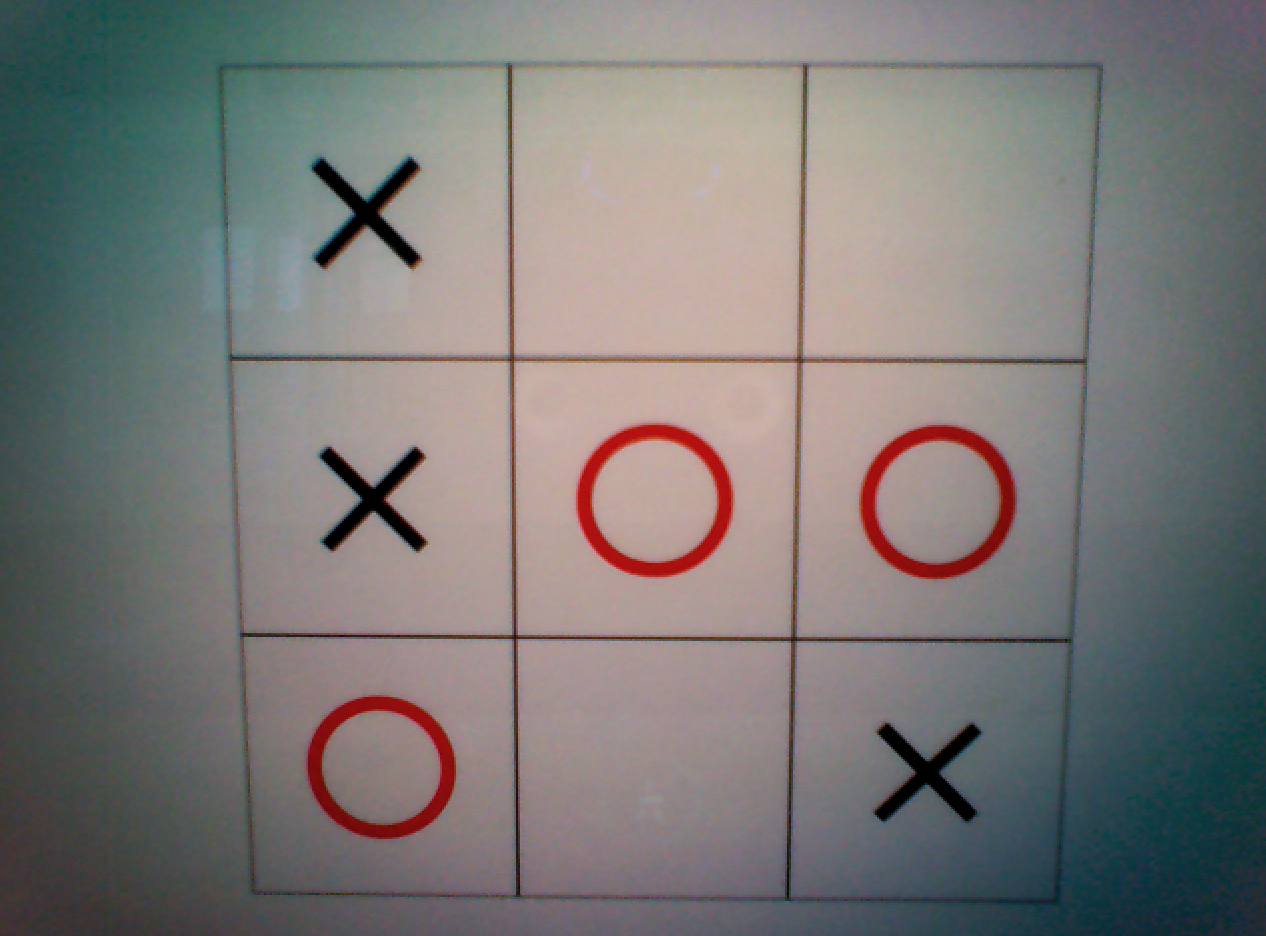
\includegraphics[width=12cm]{bilder/tictactoe_raw.png}
    \caption{\textit{TicTacToe}-Spielfeld aus Sicht des \textit{NAO}}
    \label{fig:tictactoe_raw}
\end{figure}

Wie in \ref{fig:tictactoe_raw} zu erkennen, hat die Stirnkamera des \textit{NAO} Probleme damit, ein gleichmäßig belichtetes Bild zu erzeugen. Gerade in den Ecken links oben und rechts unten zeigen sich dunklere Regionen als in der Mitte des Bildes oder links unten und rechts oben. Die Helligkeit des Tablets war bei der Aufnahme auf der höchsten Stufe. Ebenfalls erkennt man links oben und in der Mitte des Bilds Spiegelungen von Fenstern und dem Roboter selbst. Diese beiden Anomalien stellten Herausforderungen für die Bildverarbeitungsroutine dar, welche essentiell für den Erfolg der anschließenden Erkennung ist.
\begin{figure}[!htbp]
    \centering
    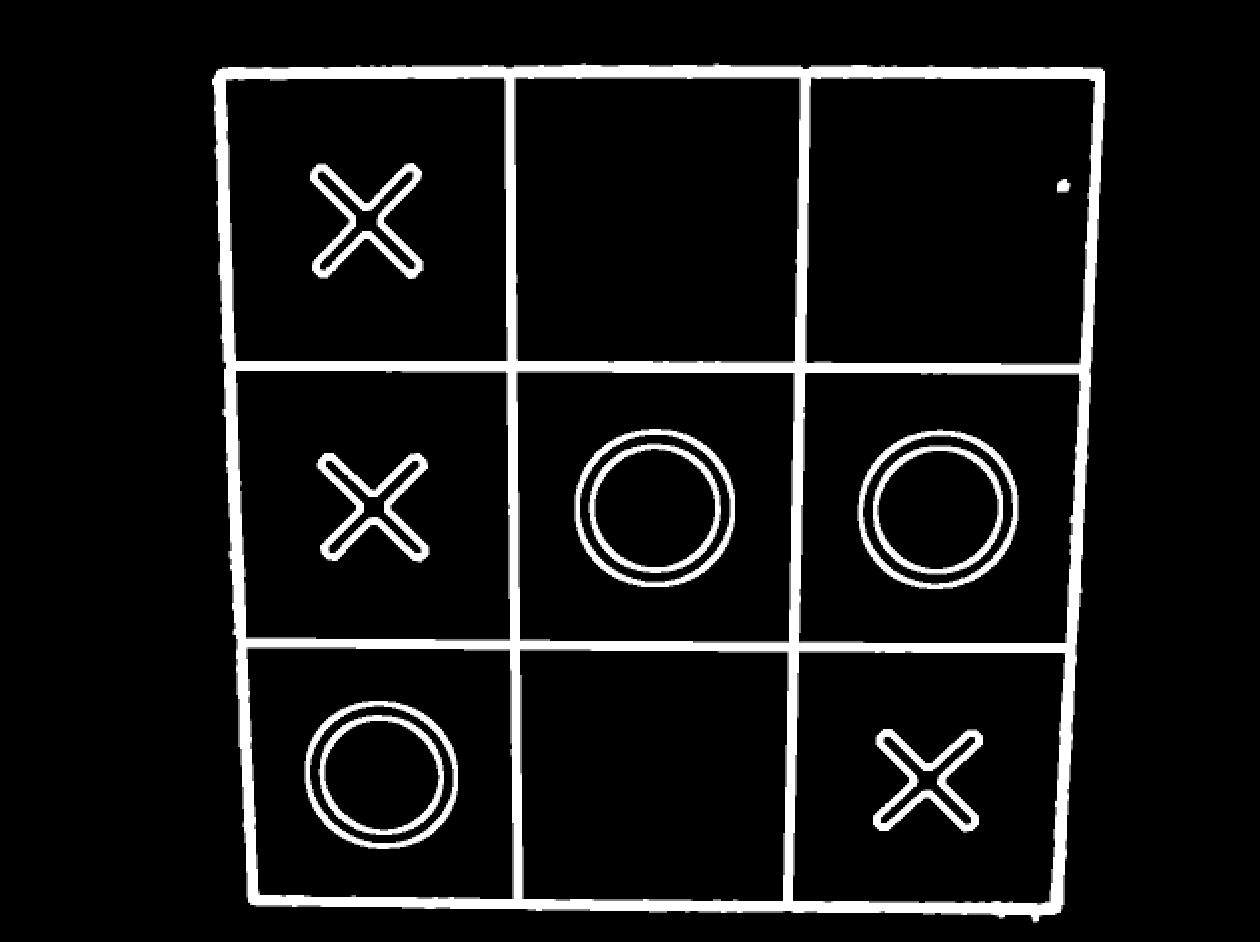
\includegraphics[width=12cm]{bilder/tictactoe_edges.png}
    \caption[\textit{TicTacToe} Kantenbild]{Nach Algorithmus \vref{image_processing_routine} und Parametern \ref{tab:vision_parameters} zu Kantenbild verarbeitetes \textit{TicTacToe}-Spielfeld}
    \label{fig:tictactoe_edges}
\end{figure}

Durch geeignete Wahl der Parameter konnten diese Störfaktoren weitestgehend entfernt werden. Lediglich im Feld rechts oben taucht ein Punkt auf, der fälschlicherweise als Kante erkannt und durch die \textit{Dilation} zusätzlich vergrößert wurde. 

\begin{figure}[!htbp]
    \centering
    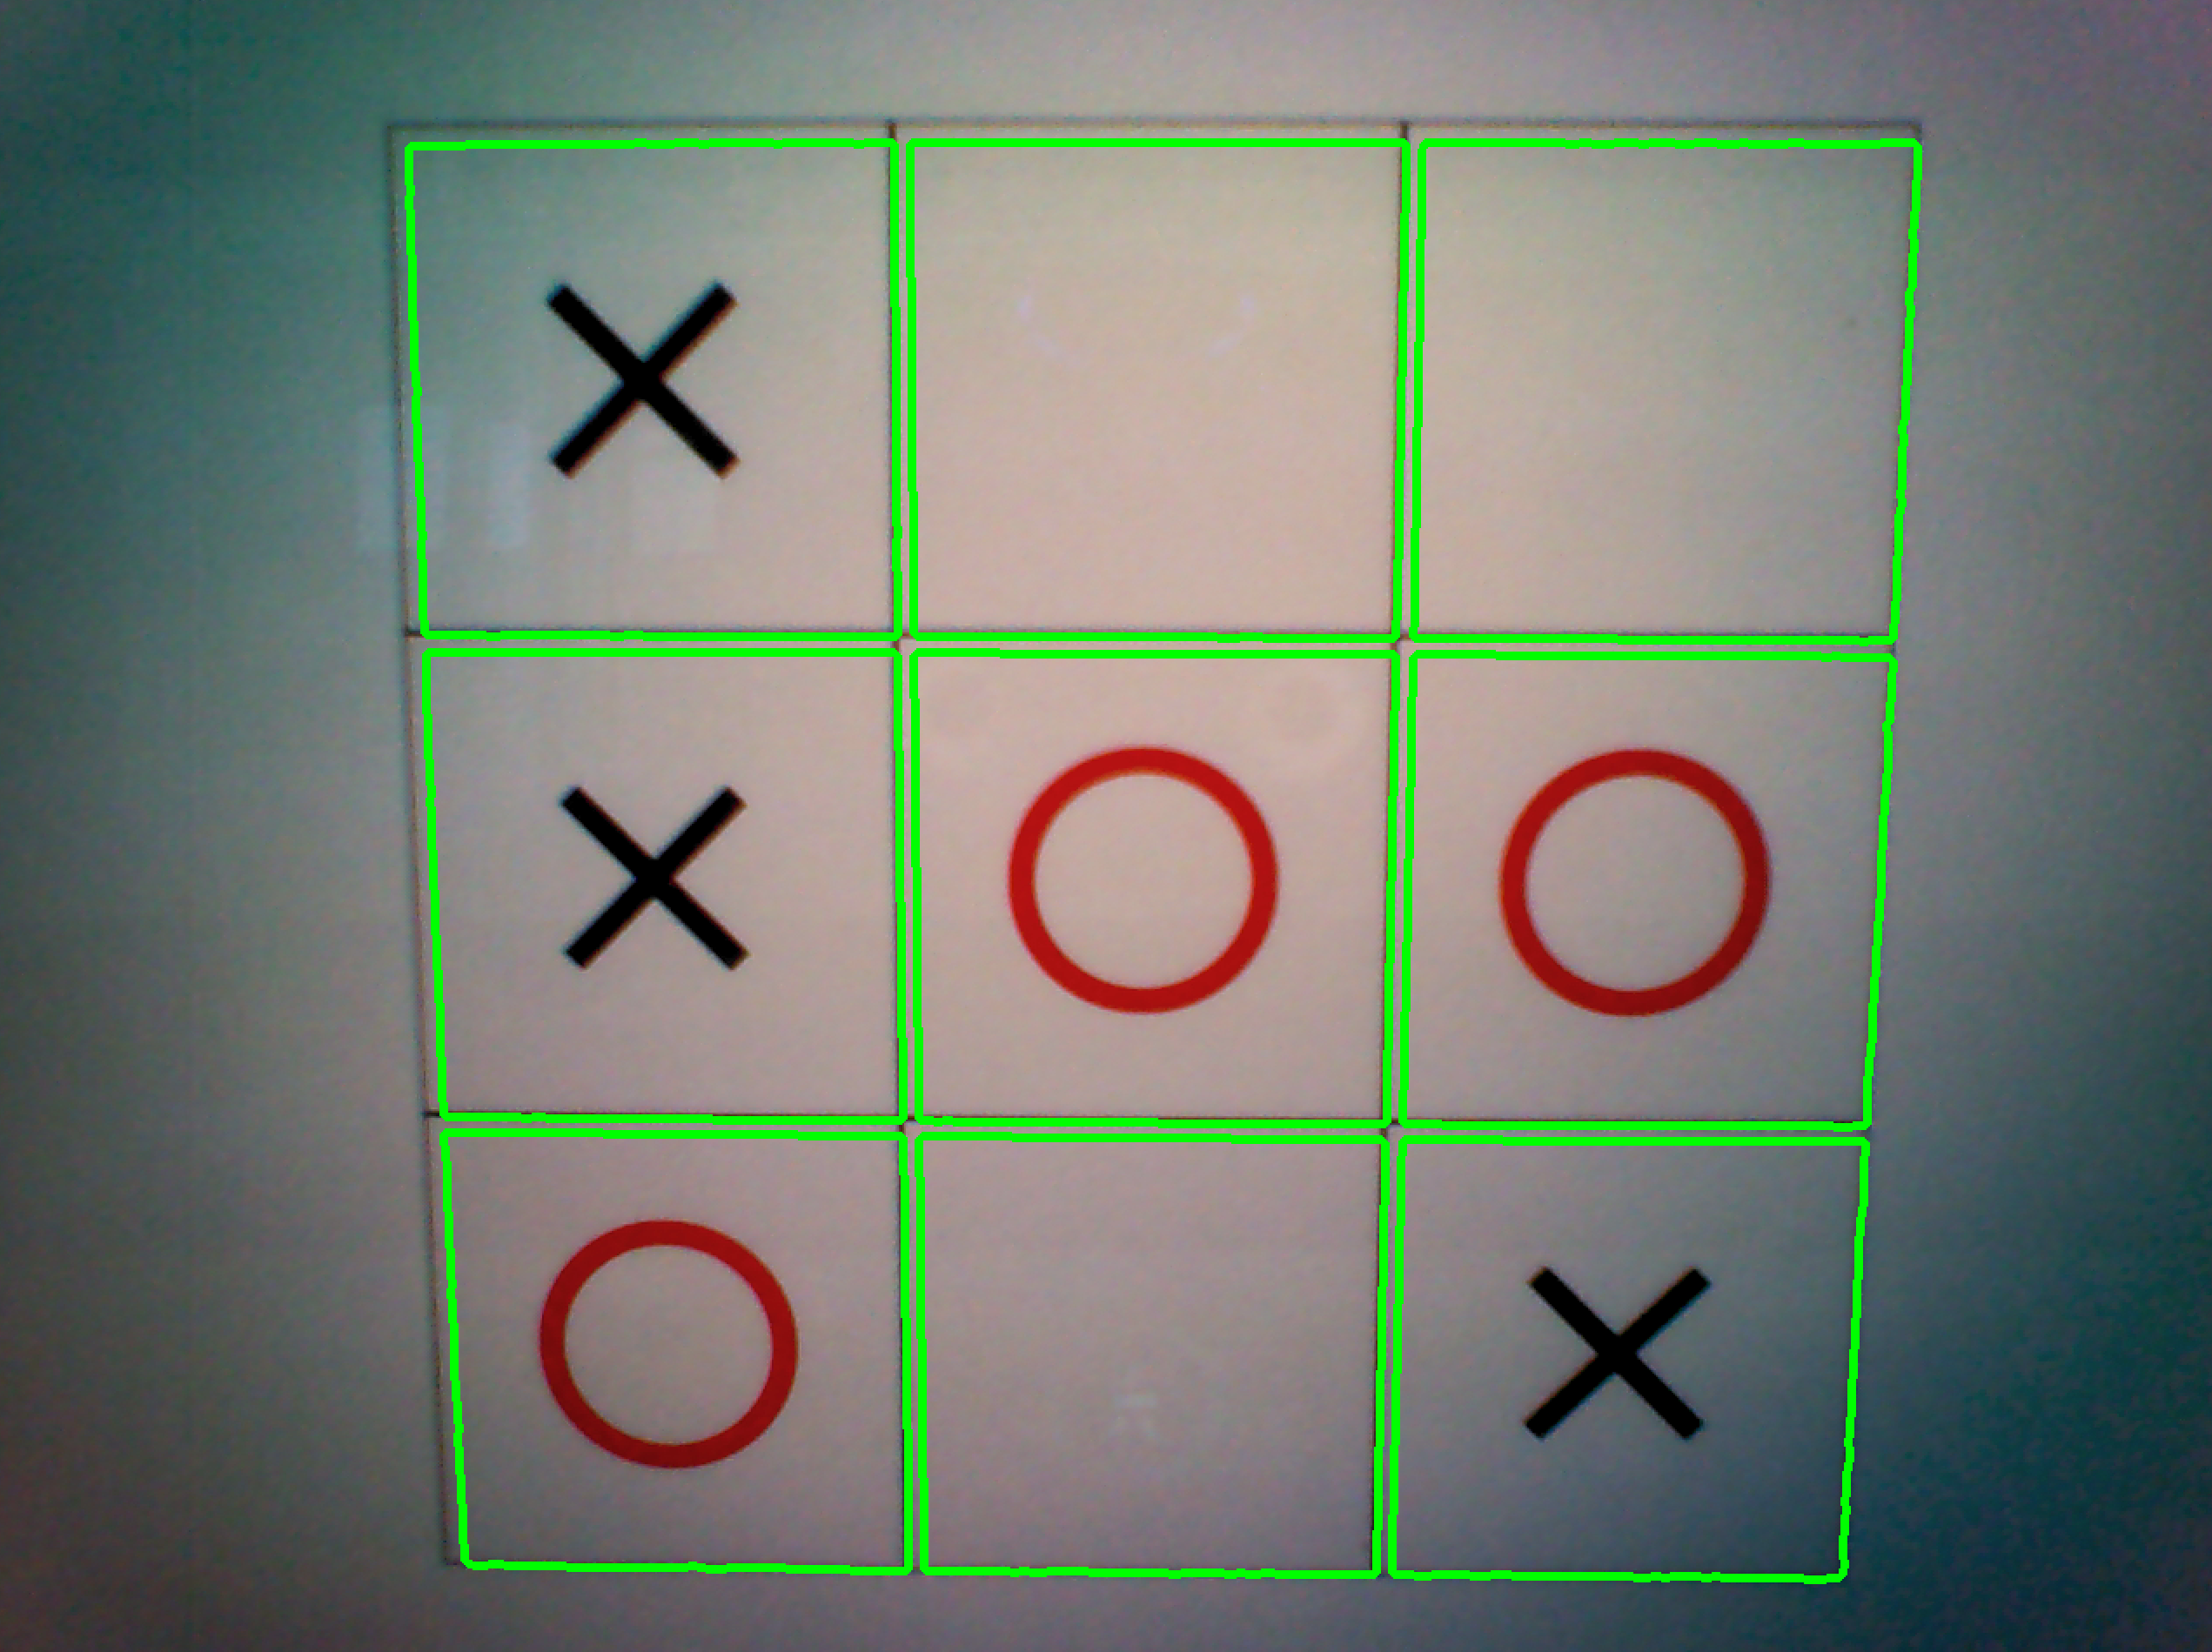
\includegraphics[width=12cm]{bilder/tictactoe_contours.png}
    \caption[\textit{TicTacToe} Konturen]{Nach Algorithmus \vref{alg:contour} erkannte Teilfelder (grün) im \textit{TicTacToe}-Spielfeld}
    \label{fig:tictactoe_contours}
\end{figure}
\noindent
Durch den Schwellenwert der Fläche der inneren Konturen, wie in \vref{alg:contour} beschrieben, werden jedoch lediglich die Ränder der Teilfelder wie gewünscht erkannt.\\

\begin{figure}[!htbp]
    \centering
    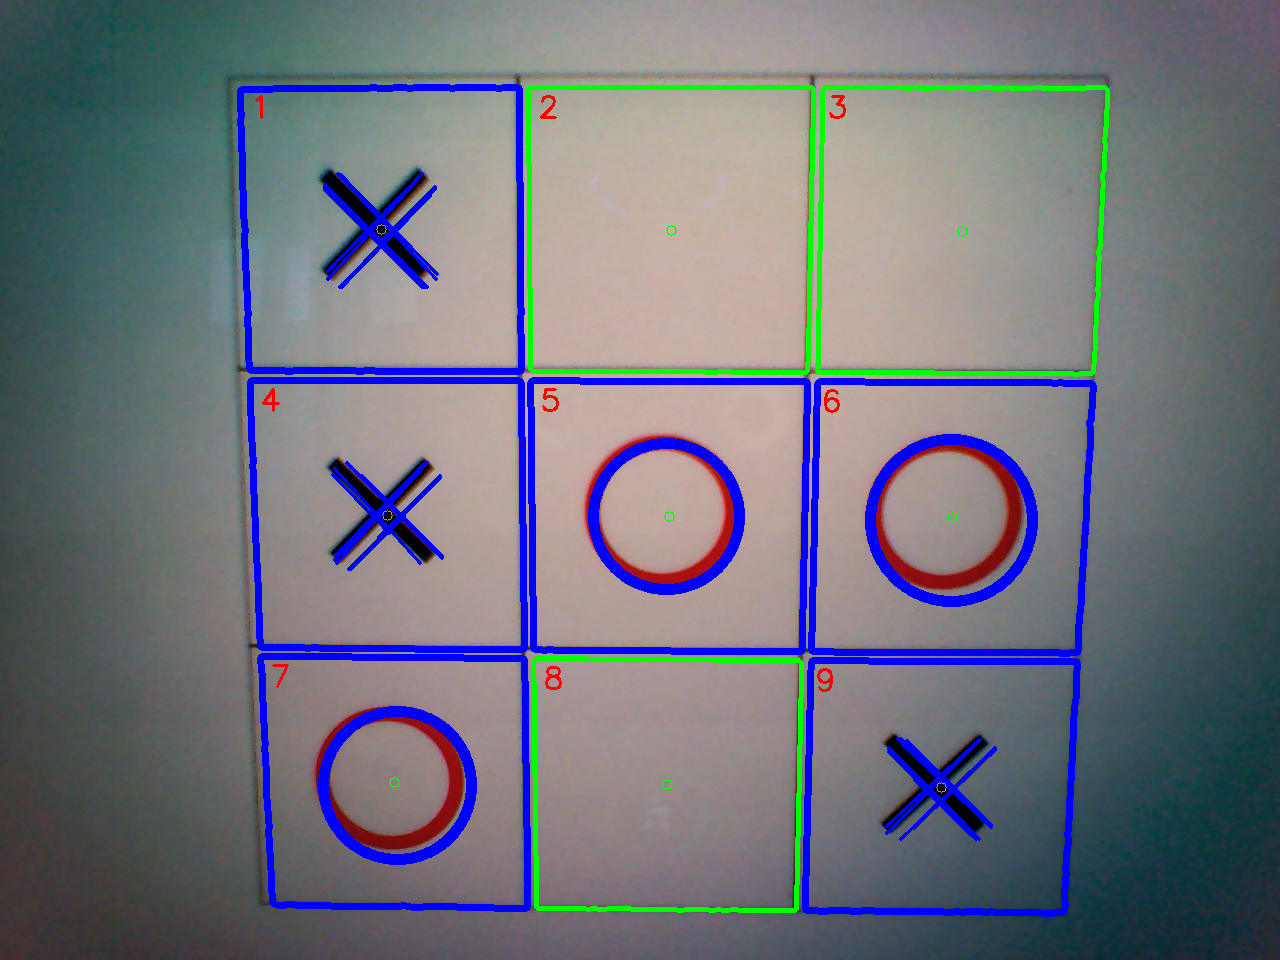
\includegraphics[width=12cm]{bilder/tictactoe_result.png}
    \caption[Ausgewertetes \textit{TicTacToe}-Spielfeld]{Nach Algorithmus \vref{alg:tictactoe_detection} erkannter Spielstand im \textit{TicTacToe}-Spielfeld, von links oben nach rechts unten nummeriert; Leere Teilfelder und Mittelpunkte in grün, Teilfelder mit Inhalt in blau.}
    \label{fig:tictactoe_result}
\end{figure}

Durch geeignete Parameter-Wahl nach \vref{tab:vision_parameters} wird der Inhalt des Spielfeldes korrekt erkannt:\\

\begin{verbatim}
    [["X", "-", "-"], 
    ["X", "O", "O"], 
    ["O", "-", "X"]]
\end{verbatim}

\newpage

\subsection{Vier gewinnt}

\begin{figure}[!htbp]
    \centering
    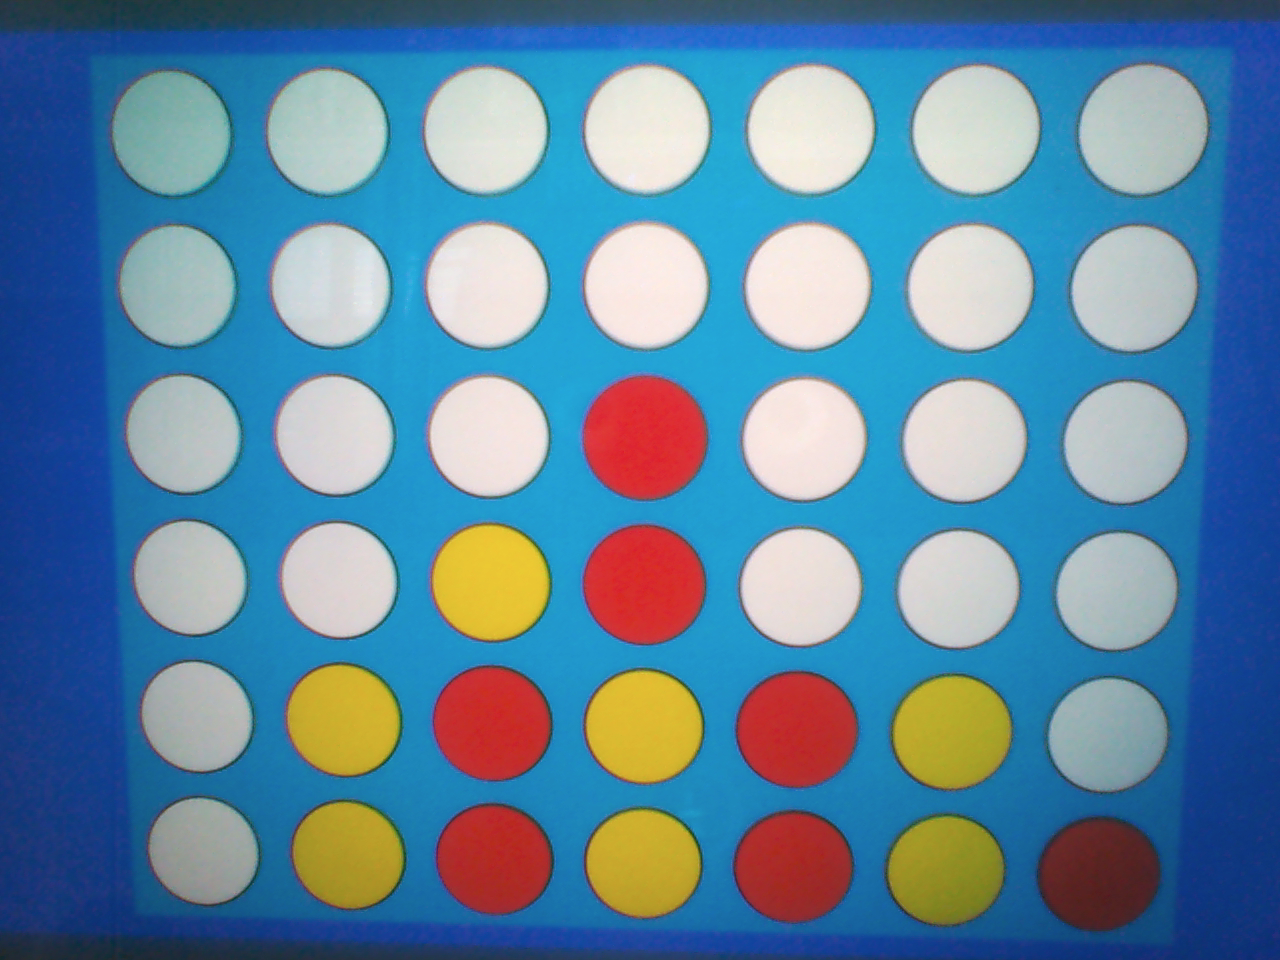
\includegraphics[width=12cm]{bilder/connect4_raw.png}
    \caption{\textit{Vier gewinnt}-Spielfeld aus Sicht des \textit{NAO}}
    \label{fig:connect4_raw}
\end{figure}

\begin{figure}[!htbp]
    \centering
    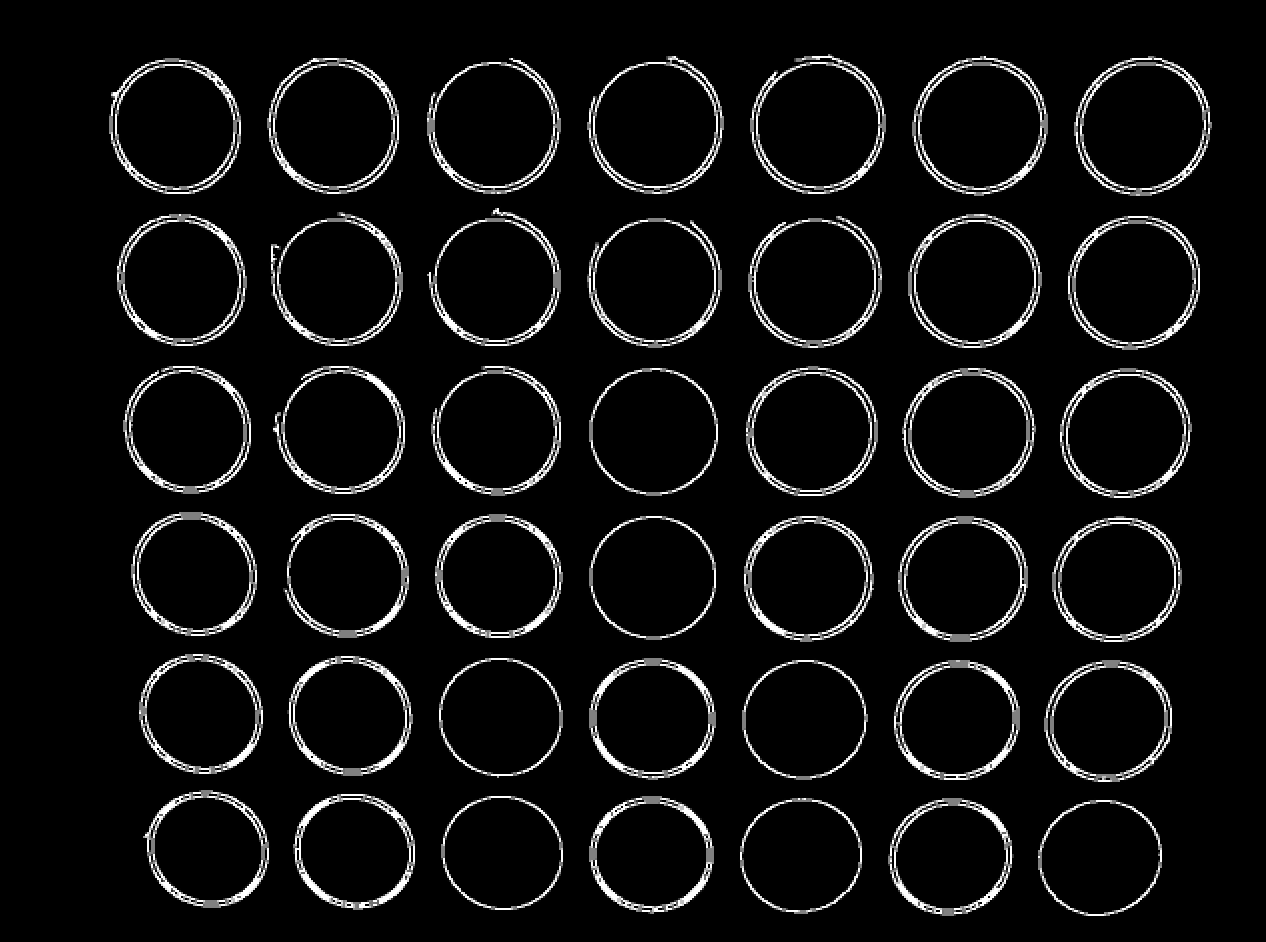
\includegraphics[width=12cm]{bilder/connect4_edges.png}
    \caption[\textit{Vier gewinnt} Kantenbild]{Nach Algorithmus \vref{image_processing_routine} und Parametern \ref{tab:vision_parameters} zu Kantenbild verarbeitetes \textit{Vier gewinnt}-Spielfeld}
    \label{fig:connect4_edges}
\end{figure}

\begin{figure}[!htbp]
    \centering
    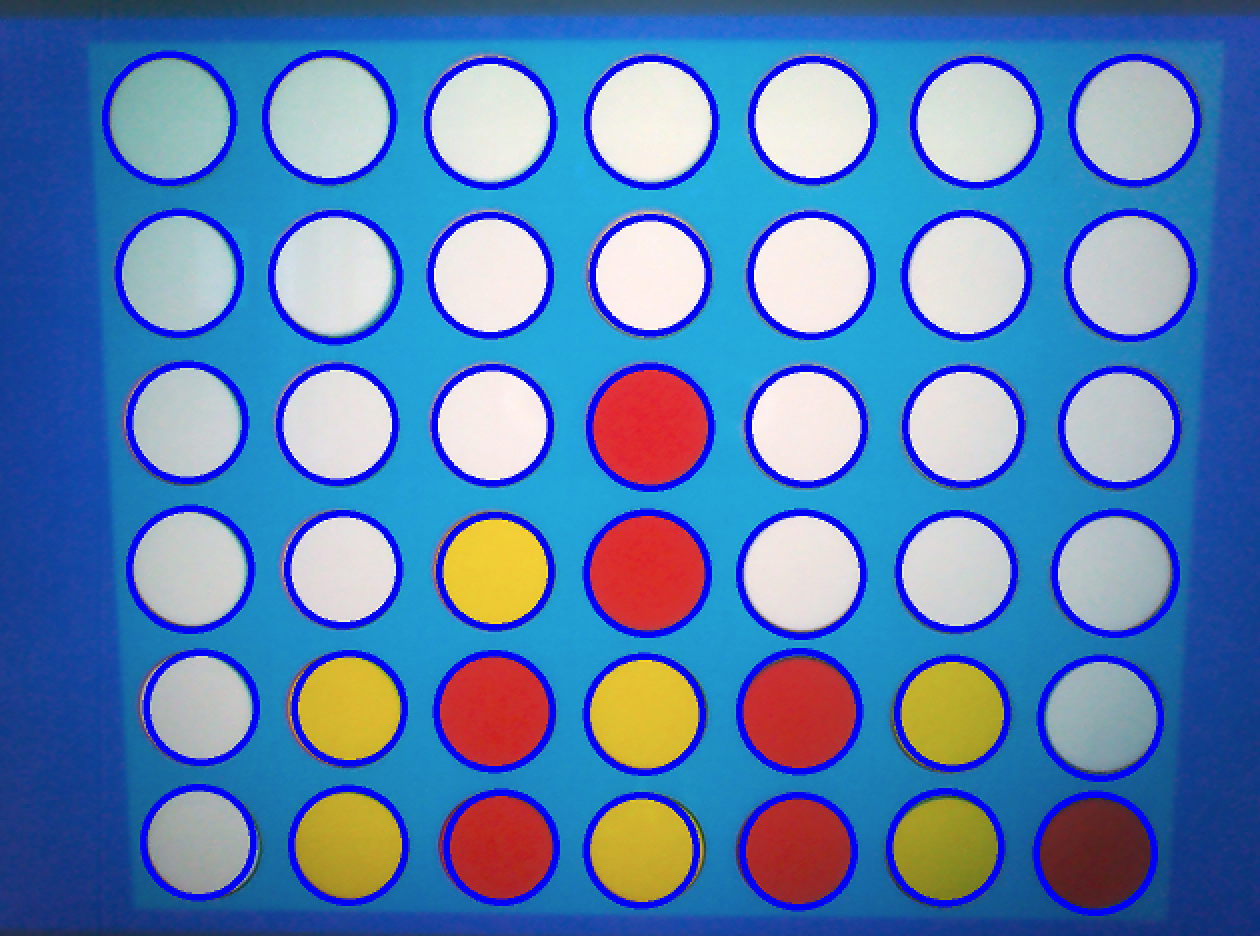
\includegraphics[width=12cm]{bilder/connect4_circles.png}
    \caption[\textit{Vier gewinnt} Kreise]{Mit Parametern \ref{tab:vision_parameters} erkannte Teilfelder im \textit{Vier gewinnt}-Spielfeld}
    \label{fig:connect4_contours}
\end{figure}

\begin{figure}[!htbp]
    \centering
    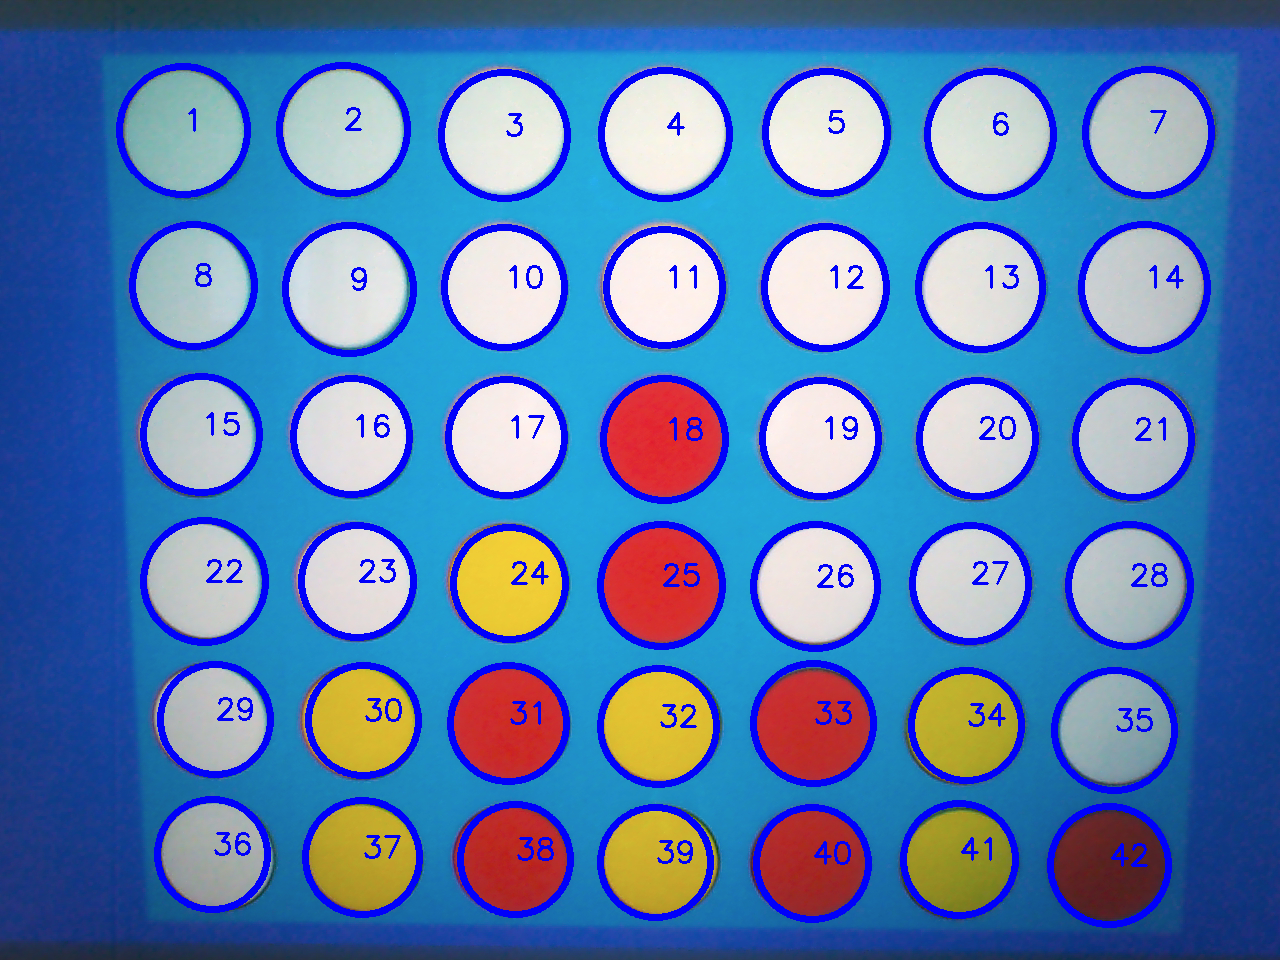
\includegraphics[width=12cm]{bilder/connect4_result.png}
    \caption[Ausgewertetes \textit{Vier gewinnt}-Spielfeld]{Nach Algorithmus \vref{alg:connect4_detection} erkannter Spielstand im \textit{Vier gewinnt}-Spielfeld}
    \label{fig:connect4_result}
\end{figure}

Durch geeignete Parameter-Wahl nach \vref{tab:vision_parameters} wird der Inhalt des Spielfeldes korrekt erkannt:\\

\begin{verbatim}
[['-', '-', '-', '-', 'R', 'Y', '-'],
['Y', 'R', '-', 'R', 'Y', 'R', 'R'],
['Y', 'R', 'Y', 'R', 'Y', 'Y', 'Y'],
['R', 'Y', 'Y', 'R', 'R', 'Y', 'Y'],
['Y', 'R', 'R', 'Y', 'R', 'Y', 'R'],
['Y', 'R', 'R', 'Y', 'Y', 'R', 'R']]
\end{verbatim}   

\subsection{Präzision}

Die Präzision der Methodik wurde anhand dieser Spielfeldkonfiguration stichprobenartig gemessen, indem standardmäßig $1000$ Bilder aufgenommen, der ermittelte mit dem tatsächlichen Spielstand verglichen und bei Unterschieden ein Zähler inkrementiert wurde. Beispiel für \textit{TicTacToe}, analog für \textit{Vier gewinnt}:

\begin{verbatim}
    def tictactoe_error_count(robotIP, PORT, field_after_move,
    iterations=1000):
    wrong_count = 0
    for i in range(iterations):
        fail = vision.get_image_from_nao(robotIP, PORT)
        field = vision.detect_tictactoe_state(fail, minRadius=65, 
        maxRadius=85, acc_thresh=15, canny_upper_thresh=25, 
        dilate_iterations=8, erode_iterations=4, 
        gaussian_kernel_size=9)
        if field != field_after_move:
            print(i)
            if field != None:
                for row in field:
                    print(row)
            wrong_count += 1
    print(wrong_count)
\end{verbatim}


\begin{verbatim}
Konfiguration 1:
[['X', '-', '-'],
['X', 'O', 'O'],
['O', '-', 'X']];
Konfiguration 2:
[['O', 'O', '-'],
['X', '-', 'X'],
['O', 'O', 'X']];
Konfiguration 3:
[['-', 'X', '-'],
['O', 'X', 'O'],
['X', 'O', 'O']];
Konfiguration 4:
[['-', '-', '-', '-', 'R', 'Y', '-'],
['Y', 'R', '-', 'R', 'Y', 'R', 'R'],
['Y', 'R', 'Y', 'R', 'Y', 'Y', 'Y'],
['R', 'Y', 'Y', 'R', 'R', 'Y', 'Y'],
['Y', 'R', 'R', 'Y', 'R', 'Y', 'R'],
['Y', 'R', 'R', 'Y', 'Y', 'R', 'R']];
Konfiguration 5:
[['-', 'R', '-', '-', '-', '-', '-'],
['-', 'Y', '-', 'Y', '-', '-', '-'],
['-', 'R', 'Y', 'R', '-', '-', '-'],
['-', 'Y', 'R', 'Y', '-', 'R', 'R'],
['R', 'R', 'R', 'Y', '-', 'Y', 'Y'],
['Y', 'Y', 'Y', 'R', '-', 'R', 'Y']];
Konfiguration 6:
[['-', '-', '-', '-', '-', '-', '-'],
['-', '-', '-', '-', '-', '-', '-'],
['-', '-', '-', '-', '-', '-', '-'],
['-', '-', '-', 'R', '-', '-', '-'],
['Y', 'R', 'R', 'Y', 'R', 'Y', '-'],
['Y', 'Y', 'R', 'R', 'Y', 'R', 'Y']];
\end{verbatim}

\begin{table}[!htbp]
\centering
\begin{tabular}{|c|c|c|c|}
  \hline
Datum & Konfiguration &  Anzahl Fehler & Anteil fehlerhafte Erkennung \\
\hline
05.09.23 & 1 & 2 & 0.002\\
\hline
11.09.23 & 2 & 2 & 0.002\\
\hline
11.09.23 & 3 & 5& 0.005\\
\hline
05.09.23 & 4 & 1 &0.001 \\
\hline
11.09.23 & 5 & 0 & 0.000\\
\hline
11.09.23 & 6 & 1 & 0.001\\
\hline

\end{tabular}
\caption{Ergebnisse für die Präzision der Spielstanderkennung von \textit{TicTacToe} und \textit{Vier gewinnt} anhand von jeweils drei Stichproben}
\label{tab:vision_parameters}
\end{table} 

Die gewählten Ansätze zur Erkennung von \textit{TicTacToe} und \textit{Vier gewinnt} erscheinen primitiv im Vergleich zu Ansätzen wie neuronalen Netzen und sind stark abhängig von der korrekten Position des Roboters vor dem Bildschirm bzw. Tablet. Jedoch wurde sich darauf geeinigt, dass sich der \textit{NAO} direkt vor dem Tablet befindet, daher konnte man von dieser Bedingung ausgehen und davon profitieren. Des Weiteren sprechen die Messungen der Präzision für den gewählten Ansatz.  Man sieht bei den Stichproben und besonders im tatsächlichen Spielablauf eine gewisse Anzahl an Fehlern. Daher sind \textit{Unit Tests} nur begrenzt möglich bzw. sinnvoll, da mit den minimal abweichenden Positionen des Roboters vor dem Bildschirm und möglichen Beleuchtungsartefakten auch keine hundertprozentige Reproduzierbarkeit garantiert ist. Somit könnten nicht bestandene \textit{Unit Tests} auftreten, welche jedoch nicht die Fehlerhaftigkeit der Methodik als solches demonstrieren und nur eine geringe Fehlerwahrscheinlichkeit besitzen. Daher zeigen diese stichprobenartigen Messungen die Zuverlässigkeit der Methodik.\\
Weitere Möglichkeiten zur Implementierung der Spielstanderkennung wären \textit{Machine}- bzw. \textit{Deep Learning} basierte Ansätze \cite{deep_learning, cascade_classifier}, oder aber Methoden wie \textit{Template Matching}, bei der Referenzbilder und der tatsächliche Input \dq verglichen\dq werden\cite{template_matching}. Zusätzlich beinhaltet \textit{naoqi} ein eigenes Bilderkennungsmodul (\textit{ALVisionRecognition}), welches ebenfalls mit Referenzbildern arbeitet. Nachteil ist hierbei jedoch, dass man Referenzbilder bzw. Trainingsdaten benötigt, welche jedoch nicht immer gleich dem aktuellen Sichtfeld des Roboters sind. Zudem können diese Ansätze potentiell rechenaufwändiger als der hier gewählte Ansatz sein, was bei dem ohnehin nicht sehr leistungsstarken Prozessor des \textit{NAO} ein Problem sein kann.